\documentclass[twocolumn, 10pt]{article}

\usepackage[margin=0.75in]{geometry}
\usepackage{amssymb,amsfonts,amsmath}
\usepackage{graphicx}

\usepackage{epstopdf}

\usepackage{natbib}

\renewcommand{\figurename}{Fig.}
\newcommand{\SI}[0]{\textit{SI Materials and Methods}}
\newcommand{\fig}[0]{Fig.}

\hyphenpenalty=10000

\makeatletter
\newcommand{\customlabel}[2]{%
\protected@write \@auxout {}{\string \newlabel {#1}{{#2}{}}}}
\makeatother

\graphicspath{{paper_figures/}}

\customlabel{fig:DV_view}{S1}
\customlabel{fig:1d_example}{S2}
\customlabel{fig:eigenvalues_drosophila_live}{S3}
\customlabel{fig:eigenvalues_zebrafish}{S4}
\customlabel{fig:eigenvalues_drosophila_fixed}{S5}
\customlabel{fig:eigenvalues_wing_disc}{S6}

\title{Temporal ordering and registration of images in studies of developmental dynamics}

\author{Carmeline~J.~Dsilva \thanks{Department of Chemical and Biological Engineering, Princeton University, Princeton, New Jersey, USA},
Bomyi~Lim \footnotemark[1],
Hang~Lu \thanks{School of Chemical and Biomolecular Engineering, Georgia Institute of Technology, Atlanta, Georgia, USA},
Amit~Singer \thanks{Department of Mathematics, Princeton University, Princeton, New Jersey, USA} \thanks{Program in Applied and Computational Mathematics, Princeton University, Princeton, New Jersey, USA},
Stanislav~Y.~Shvartsman \footnotemark[1] \thanks{Lewis-Sigler Institute for Integrative Genomics, Princeton University, Princeton, New Jersey, USA}, \\
and Ioannis~G.~Kevrekidis \footnotemark[1] \footnotemark[4]}

\date{}

\begin{document}

\maketitle

\begin{abstract}

Imaging studies provide unique insights into the dynamics of pattern formation and morphogenesis in developing tissues.
%
Developmental progress is commonly reconstructed from snapshots of chemical or mechanical processes in fixed embryos.
%
As a first step in these reconstructions, snapshots must be spatially registered and ordered in time.
%
Currently, image registration and ordering is often done manually, requiring a significant amount of expertise with a specific developmental system.
%
However, as the sizes of imaging data sets grow, these tasks become increasingly difficult, especially when the images are noisy and the examined developmental changes are subtle.
%
To address these challenges, we present an automated approach to simultaneously register and temporally order imaging data sets.
%
The approach is based on vector diffusion maps, a broadly applicable manifold learning technique that does not require \textit{a priori} knowledge of image features or a parametric model of the developmental dynamics.
%
To illustrate our approach, we register and order data from imaging studies of pattern formation and morphogenesis in three different model systems in developmental biology.

\vspace{1em}

\noindent
KEY WORDS: temporal ordering, image registration, vector diffusion maps

\end{abstract}



\section*{Introduction}

In one of the common approaches to studies of developmental dynamics, a group of embryos is fixed and stained to visualize a particular biochemical or morphological process within a developing tissue. 
%
The developmental dynamics must then be reconstructed from multiple embryos, each of which contributes only a snapshot of the relevant process along its developmental trajectory \citep{jaeger2004dynamic, peter2011gene, fowlkes2008quantitative}.
%
Importantly, the ``age'' of any given embryo arrested in its development is often only approximately known; typically what is known is
a certain time window to which a collection of embryos belongs \citep{ng2012large, richardson2014emage, castro2009automatic}.
%
Furthermore, images are often collected in different spatial orientations.
%
In order to recover the developmental dynamics from such data sets, snapshots of different embryos must first be spatially aligned or {\em registered}, and then ordered in time.
%
%We show how recently developed dimensionality reduction algorithms can automate {\it and combine} both of these tasks.


Temporal ordering and registration of images can be done manually
when the number of images is small and the differences between them are visually apparent. 
%
\fig~\ref{fig:fish} shows a caricature of fish development which illustrates the processes of growth and patterning.
%
In this case, temporal ordering can be accomplished by arranging the fish by size, which is monotonic with the developmental progress.
%
Image registration is based on obvious morphological landmarks, such as the positions of the head and the fins.
%
In contrast to this example, real data poses nontrivial challenges for both registration and temporal ordering.
%
In general, the landmarks needed for registration, as well as the attributes which can be used to order the data, are not known {\it a priori}.
%
Additional challenges arise from embryo-to-embryo variability, sample size, and measurement noise.


\begin{figure}[t]
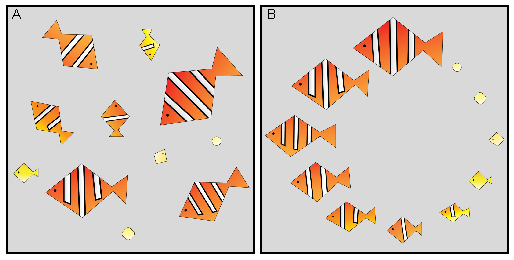
\includegraphics{fig1}
\caption{Caricature illustrating the tasks of image registration and temporal ordering. (A) Images of ``samples'', each in a different orientation and a different stage of development. (B) Registered and ordered samples. For this caricature, the registration and ordering is straightforward because the data set is small, the landmarks are visually apparent, and the developmental changes are easy to recognize.}
%\label{fig:fish}
\customlabel{fig:fish}{1}
\customlabel{subfig:fish_unordered}{\ref{fig:fish}A}
\customlabel{subfig:fish_ordered}{\ref{fig:fish}B}
\end{figure}


We present a robust algorithmic approach to registration and temporal ordering.
%
In contrast to a number of previous methodologies \citep{zitova2003image, rowley1998rotation, hajnal2010medical, greenspan1994rotation, zhao2003face}, our methodology does not rely on the {\em a priori} knowledge of spatial landmarks for registration or markers of developmental progression for temporal ordering.
%
Our approach is based on a manifold learning algorithm (vector diffusion maps \citep{singer2012vector}) which simultaneously addresses the problems of registration and temporal ordering. 
%
This algorithm is one of several nonlinear dimensionality reduction techniques that have been developed over the past decade \citep{Belkin2003, coifman2005geometric, coifman2006geometric, tenenbaum2000global, roweis2000nonlinear}, for
applications ranging from analysis of cryo-electron microscopy (cryo-EM) images of individual molecules  \citep{zhao2014rotationally, singer2011viewing} to face recognition \citep{lafon2006data} and classification of CT scans \citep{fernandez2014diffusion}.
%
Here, the vector diffusion maps algorithm is adapted for the analysis of images of developing embryos in studies of developmental dynamics, with the main objective of revealing stereotypic developmental trajectories from fixed images.
%
To illustrate our approach, we analyze four data sets common in developmental biology. 
%
Our first two data sets come from live imaging studies of {\em Drosophila} and zebrafish embryogenesis.
%
In both of these examples, the correct rotational orientation and temporal order are independently known, and these data sets will be used to validate our approach.
%from a study of {\it Drosophila} embryogenesis, one of the best experimental models for studies of development \citep{jaeger2012drosophila}.
%
Our third data set consists of images from fixed {\em Drosophila} embryos where the correct orientation and order is unknown; here, we will show how the algorithm can help uncover developmental dynamics which are not readily apparent. 
%
Our final data set consists of z-stacks of wing discs, which we will use to illustrate how our methods extend to three-dimensional imaging. 
%
We will also show how to compute an average trajectory from a set of registered and ordered fixed images to remove noise due to intersample variability and obtain a smooth description of the underlying developmental dynamics. 

\section*{Results}

\subsection*{Vector diffusion maps for registration and temporal ordering}

Vector diffusion maps \citep{singer2012vector} is a manifold learning
technique developed for data sets which contain two sources of variability:
geometric symmetries (such as rotations of the images) which one would like to factor out,
and ``additional" directions of variability (such as temporal dynamics) which one would like to uncover.
%
Vector diffusion maps combine two algorithms, {\em angular synchronization} \citep{singer2011angular} for image registration and {\em diffusion maps} \citep{coifman2005geometric} for extracting intrinsic low-dimensional structure in data, into a single computation.
%
We will use the algorithm to register images of developing embryos with respect to rotations, as well as uncover the main direction of variability {\it after} removing rotational symmetries.
%
Although in general, images may contain variations due to rotations, translations, and scaling, we will remove relevant translations and/or scaling via relatively simple preprocessing, and focus only on factoring out rotations using the vector diffusion maps algorithm.
%
In the case that all relevant symmetries can be removed with straightforward preprocessing procedures, our algorithms can also be used simply to extract the main direction of variability within the imaging data set. 
%
We assume that the main direction of remaining variability in these images is parameterized by the developmental time of each embryo.
%
As a consequence, uncovering this direction should reveal the underlying developmental dynamics.

\begin{figure}[t]
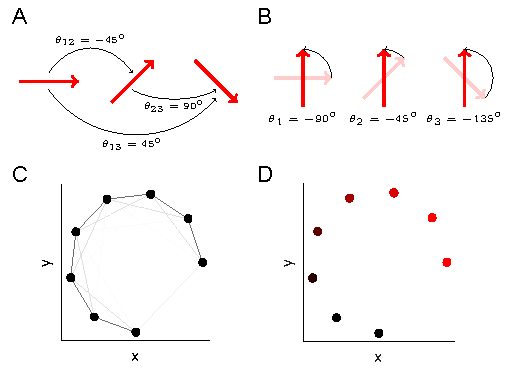
\includegraphics{fig2}
\caption{Schematic illustrating angular synchronization and diffusion maps. (A) Set of vectors, each in a different orientation. The pairwise alignment angles are indicated. (B) The vectors from A, each rotated about their midpoint so that the set is globally aligned. Note that the chosen rotation angles are consistent with the pairwise alignments in A: the differences between a pair of angles in B is the same as the pairwise angle in A. (C) Data points (in black) which lie on a one-dimensional nonlinear curve in two dimensions. Each pair of points is connected by an edge, and the edge weight is related to the Euclidean distance between the points through a Gaussian kernel (see \SI), so that close data points are connected by darker (``stronger'') edges. (D) The data in C, colored by the first (non-trivial) eigenvector from the diffusion map computational procedure. The color intensity is monotonic with the perceived curve arclength, thus parameterizing the curve.}
\label{fig:schematics}
\end{figure}

Angular synchronization uses pairwise alignment information to register a set of images in a globally consistent way.
%
A schematic illustration of angular synchronization is shown in \fig~\ref{fig:schematics}A, where each image is represented as a vector, and the goal is to align the entire set of vectors given pairwise alignment measurements.
%
We first compute the angles needed to align pairs of vectors (or images), which in general requires no template function \citep{ahuja2007template}.
%
In this work, we aligned pairs of images with respect to rotations by exhaustively searching over a discretized space of rotation angles. 
%
However, in other applications, pairwise alignments can be computed by aligning appropriate image landmarks or features. 
%
When the data are noisy, these pairwise measurements may by inaccurate, and so we would like to utilize {\em all} pairwise measurements to align the set of images robustly. 
%
Using the alignment angles between all pairs of vectors, angular synchronization finds the set of rotation angles (one angle for each vector) that is most consistent with {\it all} pairwise measurements (see \SI); this is illustrated in \fig~\ref{fig:schematics}B.
%
In this schematic, registration via angular synchronization is trivial, as the pairwise measurements contain no noise.
%
However, the algorithm can successfully register data sets even when many of the pairwise measurements are inaccurate \citep{singer2011angular}.

After removing variability due to rotations, the developmental dynamics may be revealed by ordering the data along the one-dimensional manifold that parameterizes most of the remaining variability in the data.
%
Such a manifold can be discovered using diffusion maps \citep{coifman2005geometric}, a nonlinear dimensionality reduction technique that uncovers an intrinsic parameterization of data that lies on a low-dimensional manifold in high-dimensional space.
%
The idea is illustrated in \fig~\ref{fig:schematics}C, where the data are two-dimensional points which lie on a one-dimensional nonlinear curve.
%
We use {\it local} information about the data to find a parameterization which respects the underlying manifold geometry, so that points which are close in high-dimensional space (e.g., images which look similar) are close in our parameterization.
%
This idea of locality is denoted by the color of the edges in \fig~\ref{fig:schematics}C:
data points which are close are connected by dark edges, and clearly, the dark edges are more ``informative" about the low-dimensional structure of the data.
%
The color in \fig~\ref{fig:schematics}D depicts the one-dimensional parameterization or ordering of the data that we can detect visually.
%
In our working examples, each data point will be of much higher dimension (e.g., a pixelated image or three-dimensional voxel data), and so we cannot extract this low-dimensional structure visually.
%
Instead, we will use diffusion maps to automatically uncover a parameterization of our high-dimensional data (see \SI).
%
Diffusion maps generalizes directly from one-dimensional nonlinear curves to higher-dimensional manifolds.


\subsection*{Method validation using live imaging}

\subsubsection*{{\em Drosophila} gastrulation}

\begin{figure*}[t]
\raisebox{0.75cm}{\textsf{A}}
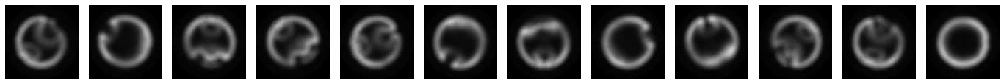
\includegraphics[width=17cm]{drosophila_live_imaging_scrambled}

\raisebox{0.75cm}{\textsf{B}}
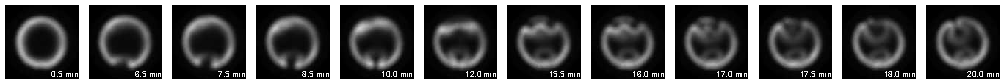
\includegraphics[width=17cm]{drosophila_live_imaging_ordered}

\raisebox{4.25cm}{\textsf{C}}
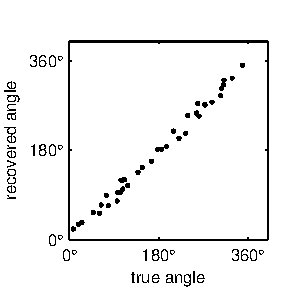
\includegraphics[width=5cm]{drosophila_live_imaging_angle_corr}
%
%\hfill
%
\raisebox{4.25cm}{\textsf{D}}
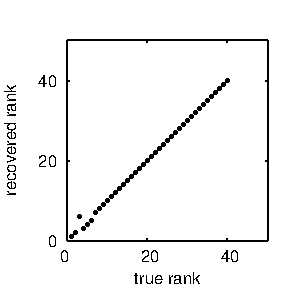
\includegraphics[width=5cm]{drosophila_live_imaging_rank_corr}
%
%\hfill
%
\raisebox{4.25cm}{\textsf{E}}
%
\raisebox{2.5cm}{
{ \textsf{ 
\begin{tabular}{ |c | c| c| }
\hline
\parbox[c]{1.5cm}{ \centering Movie Index} & \parbox[c]{1.5cm}{ \vspace{.5\baselineskip} \centering Average Angle Error \vspace{.5\baselineskip}} & \parbox[c]{1.5cm}{ \centering Rank Correlation Coefficient} \\
\hline
1 & 8.37$^{\circ}$ & 0.9989 \\ 
2 & 4.98$^{\circ}$ & 0.9994 \\ 
3 & 6.47$^{\circ}$ & 0.9795 \\ 
4 & 7.03$^{\circ}$ & 0.9953 \\ 
5 & 3.04$^{\circ}$ & 0.9959 \\ 
 \hline
\end{tabular}}}}
\caption{Method validation using live imaging of \textit{Drosophila} embryos. (A) Selected images from a live imaging study of a \textit{Drosophilla} embryo during gastrulation. Each frame is in an arbitrary rotational orientation, and the order of the frames has been shuffled. (B) Images from A after registration and ordering using vector diffusion maps. The dorsal side of each embryo now appears at the top of each image, and the ventral side appears at the bottom. (C) The correlation between the recovered rotation angle (using vector diffusion maps) and the true rotation angle. The average absolute error in the recovered angles is $8.37 ^\circ$. (D) The correlation between the recovered rank (using vector diffusion maps) and the true rank. The rank correlation coefficient is $0.9989$. (E) The average error in the recovered angle and the rank correlation coefficient for $5$ different live imaging studies. }
\label{fig:drosophila_live_imaging}
\end{figure*}

To validate the proposed approach, we applied our algorithm to a data set where the true temporal order and rotational orientation of the images were known {\em a priori}.
%
This data set was obtained through live imaging near the posterior pole of a vertically oriented {\it Drosophila} embryo during the twenty minutes spanning the late stages of cellularization through early gastrulation.
%
During this time window, the ventral furrow is formed, where the ventral side buckles towards the center of the embryo, internalizing the future muscle cells and forming a characteristic ``omega'' shape.
%
Germband extension then causes cells from the ventral side to move towards the posterior pole of the embryo, and then wrap around to the dorsal side \citep{leptin2005gastrulation}.
%
At the end of this process, cells which were originally on the ventral and posterior side of the embryo find themselves on the dorsal side, causing a similar ``omega'' to appear on the dorsal side.

\fig~\ref{fig:drosophila_live_imaging}A shows selected images from this live imaging data set, which contains $40$ consecutive frames taken at $30$~second time intervals at a fixed position within a single embryo.
%
Each image shows an optical cross-section near the posterior pole of a vertically oriented developing embryo, with the nuclei labeled by Histone-RFP.
%
Each frame was arbitrarily rotated, and the order of the frames was scrambled.
%
The task is now to register these images and order them in time to reconstruct the developmental trajectory.

We used vector diffusion maps to register and order the images. 
%
\fig~\ref{fig:drosophila_live_imaging}B shows the images from \fig~\ref{fig:drosophila_live_imaging}A, now registered and ordered; the real time for each frame is also indicated.
%
With a small number of exceptions, the recovered ordering is consistent with the real time dynamics. 
%
\fig~\ref{fig:drosophila_live_imaging}C and \fig~\ref{fig:drosophila_live_imaging}D  show the correlations between the recovered and true angles and ranks, respectively, for the entire data set. 
%
Both the angles and the ranks are recovered with a high degree of accuracy.

To assess the robustness of our proposed methodology, we repeated this procedure with four additional data sets extracted from independent live imaging studies spanning the same developmental time period. 
%
The results are shown in \fig~\ref{fig:drosophila_live_imaging}E. 
%
The errors in the recovered angles are all less than 10$^\circ$, and the rank correlation coefficients are consistently greater than 95\%, indicating that our methodology can reproducibly order data of this type. 

In general, to accurately recover the temporal order, the vector diffusion maps algorithm requires a sufficient amount of data so that the underlying one-dimensional curve (i.e., the curve in \fig~\ref{fig:schematics}C) is well-sampled.
%
At the same time, the accuracy of the recovered alignments is a function of the signal-to-noise ratio in the pairwise alignments, as well as the size of the data set \citep{singer2011angular}.
%
%Clearly, $40$ images are sufficient to accurately recover the rotational orientation and temporal order in this specific developmental time frame.
%%
%To quantitatively assess how our methods perform as a function of sample size, we used bootstrap sampling to compute the rank correlation as a function of the size of the data set.
%%
%Subsets of images were randomly selected from the $40$-image data set, and then registered and ordered. 
%%
%\fig~\ref{subfig:movie_bootstrap} shows the median rank correlation coefficient as a function of the number of images in the subset.
%%
%As expected, the accuracy in the recovered ordering increases with the number of images. 
%% 
%At the same time, we see that correct order is recovered even with a relatively small number of snapshots, which should make our approach applicable other studies of developmental processes.
%%
Because our particular data set contains relatively low noise levels, few images were required to obtain accurate rotational alignment, and the high temporal resolution of our live imaging study allows us to order the images accurately.  
%
In summary, the algorithm accurately and robustly registers and orders a model data set where both the rotation angles and real times are independently known. 

\subsubsection*{Zebrafish gastrulation}

\begin{figure*}[t]
\begin{minipage}[c]{13.75cm}
\vspace{0cm}
\raisebox{0.5cm}{\textsf{A}}
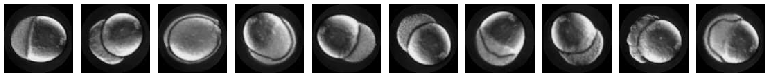
\includegraphics[width=13cm]{zebrafish_scrambled}

\raisebox{0.5cm}{\textsf{B}}
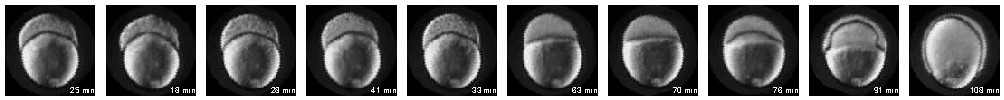
\includegraphics[width=13cm]{zebrafish_ordered}
\end{minipage}
%
\hfill
%
\begin{minipage}[c]{3.75cm}

\vspace{0cm}
\raisebox{2.5cm}{\textsf{C}}
%
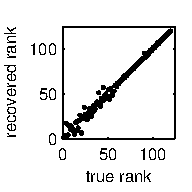
\includegraphics[width=3.25cm]{zebrafish_rank_corr}
\end{minipage}
\caption{Method validation using live imaging of a zebrafish embryo. (A) Selected images from a flip book movie of zebrafish embryogenesis. Each frame is in an arbitrary rotational orientation, and the order of the frames has been shuffled. (B) Images from A after registration and ordering using vector diffusion maps. The real time of each frame is also indicated. (C) Correlation between the rank recovered using vector diffusion maps and the true rank.  The rank correlation coefficient is $0.9954$. The larger errors in the recovered ranks towards the beginning of the trajectory are due to the rather static cell movement within that time window. }
\label{fig:zebrafish}
\end{figure*}


To illustrate the broad applicability of our approach, we also applied our algorithm to a time-lapse movie  of zebrafish embryogenesis. 
%
We used a publicly available flipbook movie of zebrafish embryogenesis, available at \texttt{https://zfin.org/zf\_info/movies/Zebrafish.mov} \citep{karlstrom1996flipbook}.  
%
Taken with a differential interference contrast (DIC) microscope, the movie records the first $17$~hours of zebrafish development, from a single cell stage to a 16-somite stage. 
%
We selected $120$ consecutive frames from this movie which capture 5.5~hours of epiboly (3.5--9~hours after fertilization). 
%
At the start of the time window, cells have divided 10--11 times and are accumulated in a cell mass above the yolk. 
%
The cell mass is then compressed and the animal-vegetal axis of the embryo (vertical axis in the \fig~\ref{fig:zebrafish}) shortens to form a spherical embryo shape by the end of the fourth hour of development. 
%
Then, the yolk syncytial layer, which forms the boundary between the yolk and the cell mass, moves upward, forming a dome-shaped structure.  
%
During this stage, the cells rearrange to form a cell layer with uniform thickness (about four cells thick). 
%
With time, this cell layer then spreads over across the yolk and expands toward the vegetal pole. 
%
At the end of epiboly, the blastoderm completely engulfs the yolk. 

As in the example of {\em Drosophila} embryo live imaging, the frames were randomly rotated and shuffled (\fig~\ref{fig:zebrafish}A). 
%
We then used vector diffusion maps to register and order the frames. 
%
The results are shown in \fig~\ref{fig:zebrafish}B. 
%
The recovered rotations and order are consistent with the expected developmental dynamics, as shown in the correlations between the recovered and true ranks (\fig~\ref{fig:zebrafish}C). 
%
Quantitatively, the rank correlation coefficient for this data set is 0.9954, and the average error in the recovered angle is $4.14^\circ$. 
%
Some errors in ordering images of the early embryo result from rather static cell movement during the early developmental stage where cells divide and accumulate above the yolk. 
%
During epiboly, cell movement is more dynamic and the recovered ordering is more consistent with the real dynamics.


In summary, we showed that our algorithm is not limited to a specific set of data. 
%
The algorithm works for different tissue types ({\em Drosophila} and zebrafish), and also for images taken with different imaging methods (fluorescent and phase contrast images).
%
Provided there exist significant dynamics within the data set and that the developmental trajectory is well-sampled, the developmental dynamics can be recovered.

\subsection*{Data sets with intersample variability}

\subsubsection*{Fixed {\em Drosophila} images}

\begin{figure*}[t]
\begin{minipage}[b]{12cm}
\raisebox{0.5cm}{\textsf{A}}
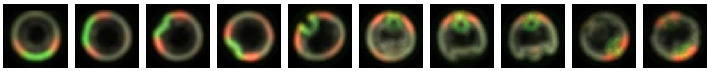
\includegraphics[width=12.25cm]{drosophila_fixed_images_scrambled}

\raisebox{0.5cm}{\textsf{B}}
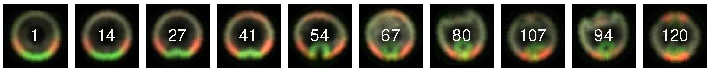
\includegraphics[width=12.25cm]{drosophila_fixed_images_ordered}

\raisebox{0.5cm}{\textsf{C}}
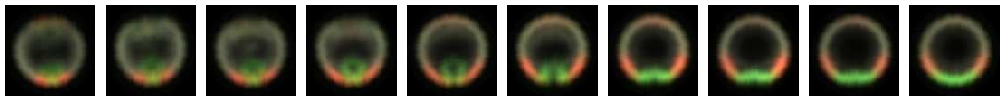
\includegraphics[width=12.25cm]{drosophila_fixed_images_average}
\end{minipage}
%
\hfill
%
\raisebox{3.25cm}{\textsf{D}}
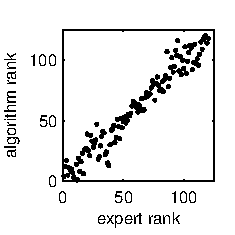
\includegraphics[width=4.25cm]{drosophila_fixed_images_rank_corr}
%
\caption{Analyzing images of fixed \textit{Drosophila} embryos. {(A)} Images of \textit{ Drosophila} embryos, stained for nuclei (gray), Twi (green), and dpERK (red). Each image is of a different embryo arrested at a different developmental time and in a different rotational orientation. {(B)} Data from {\it A}, registered and ordered using vector diffusion maps. The expert rank for each image is indicated. {(C)} A representative ``developmental trajectory'' obtained from local averaging of the entire set of registered and ordered images (see \SI). {(D)} Correlation between the image ranks calculated from the vector diffusion maps algorithm and the ranks obtained from ordering by an expert. The rank correlation coefficient is $0.9716$. }
\label{fig:drosophila_fixed_images}
\end{figure*}


We have analyzed how our algorithm performs on two model data sets where all images come from a single embryo. 
%
In practice, we are interested in cases where image comes from a different embryo, and the largest source of noise in the considered data set arises from embryo-to-embryo variability.
%
To demonstrate that our methods are robust to such noise sources,
we constructed a synthetic time course data set by selecting a random image from one of five {\em Drosophila} live imaging data sets (those data sets used in \fig~\ref{fig:drosophila_live_imaging}) at each time point.
%
The resulting data set is spatially unregistered, scrambled in time, and reflects embryo-to-embryo variability. 
%
The median rank correlation coefficient when ordering such a synthetic time course using our methodology was 0.77, indicating that the algorithm can accurately recover the temporal order even under noisy conditions. 

We then applied our approach to a data set where the true rotational orientation and temporal order was not known {\it a priori}.
%
\fig~\ref{fig:drosophila_fixed_images}A shows selected images from a set of $120$ images of developing {\em Drosophila} embryos which cover a thirty minute time interval spanning late cellularization through gastrulation.
%
This data set is more complex than the live imaging data sets in that it contains significantly more images, each of which provides information about tissue morphology and the spatial distribution of two regulatory proteins.
%
Each image shows an optical cross-section of the posterior view of a {\em different} embryo at a different rotational orientation and fixed at a different (and unknown) developmental time.
%
The nuclei (gray) were labeled with DAPI, a DNA stain.
%
Embryos were stained with the antibody that recognizes Twist (Twi, shown in green), a transcription factor which specifies the cells of the future muscle tissue.
%
Another signal is provided by the phosphorylated form of the extracellular signal regulated kinase (dpERK, shown in red), an enzyme that, in this context, specifies a subset of neuronal cells \citep{Lim2013kinetics}.

\fig~\ref{fig:drosophila_fixed_images}B shows the selected images in \fig~\ref{fig:drosophila_fixed_images}A, now registered and ordered using vector diffusion maps \citep{singer2012vector}.
%
However, because of interembryo variability, these selected images are not entirely representative of the developmental dynamics across the entire data set.
%
To highlight the developmental dynamics revealed by vector diffusion maps, we computed an average developmental trajectory across the set of registered and ordered images (see \SI). 
%
Each snapshot in the average trajectory is the (weighted) average of a group of successive images from the registered and ordered data set.
%
Averaging successive images removes (some) of the interembryo variability, so that sequential snapshots of this averaged trajectory, shown in \fig~\ref{fig:drosophila_fixed_images}C, serve as a summary of the stereotypic developmental dynamics.

From this average trajectory, we can now easily see the developmental progression, which is consistent with the known dynamics: 
dpERK first appears as two lateral peaks at the ventral side of the embryo; a third dpERK peak then appears at the dorsal side of the embryo.
%
During mesoderm invagination, the two ventral dpERK peaks merge together, eventually forming, together with Twi, the ``omega'' shape.
%
The dorsal dpERK peak then disappears during germband extension as cells from the ventral side wrap around to the dorsal side.
%
At the end of this process, similar ``omegas'' formed by Twi and dpERK appear on the dorsal side of the embryo; these patterns are most readily seen in the last image of \fig~\ref{fig:drosophila_fixed_images}C.
%
Thus, vector diffusion maps can accomplish the tasks presented in the caricature in \fig~\ref{fig:fish}, even in the absence of information about image landmarks (e.g., fins) and without {\it a priori} knowledge of developmental features (e.g., correlation of age with body size).
%

To evaluate the quality of our registration and ordering, we can use prior knowledge about the developmental system. 
%
The Twi signal is known to form a single peak at the ventralmost point of the embryo. 
%
We found that the standard deviation in the location of this peak in the set of registered images was $\sim$8$^\circ$,
indicating that the algorithm successfully aligns the ventralmost points of the images. 
%
Because the developmental time of each embryo cannot be easily estimated, we have few options for evaluating the quality of our temporal ordering. 
%
We compared the ordering obtained from vector diffusion maps to the ordering provided by a trained embryologist who is knowledgeable about the developmental progression and the important image features.  
%
The ranks from the ordering provided by the embryologist, which we will refer to as the ``expert rank'', are indicated for the images in \fig~\ref{fig:drosophila_fixed_images}B , and the rank correlation (see \fig~\ref{fig:drosophila_fixed_images}D) shows that our ordering is consistent with the expert ordering. 


\subsubsection*{Wing disc data}

\begin{figure*}[t]
\raisebox{5.5cm}{\textsf{A}}
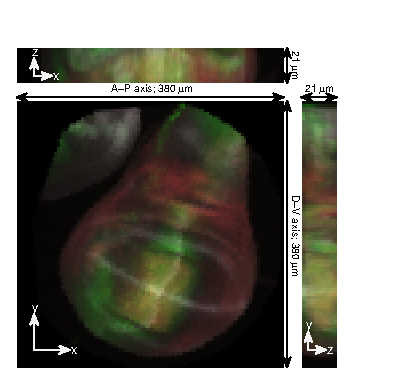
\includegraphics[width=6cm]{wing_disc_example}
%
\hfill
%
\raisebox{5.5cm}{\textsf{B}}
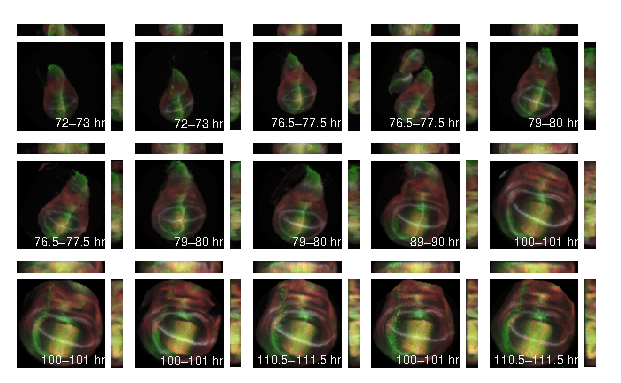
\includegraphics[width=10cm]{wing_disc_ordered}

\vspace{0.25cm}
\raisebox{2.25cm}{\textsf{C}}
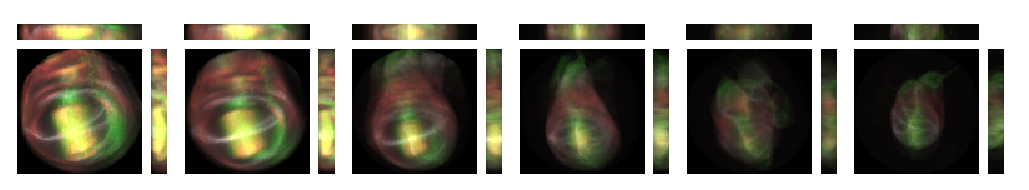
\includegraphics[width=17.5cm]{wing_disc_average}

\caption{Three-dimensional wing disc data. (A) Maximum projections of an example three-dimensional image. Projections along the $x$-, $y$-, and $z$-axes are shown. (B) Example three-dimensional images, ordered using diffusion maps. The time cohort, as assessed by an expert, is indicated for each image, and the rank correlation coefficient between the diffusion maps ordering and the expert timing is 0.9427. (C) The average developmental trajectory for the registered and ordered images. }
\label{fig:wing_disc}
\end{figure*}

We have demonstrated that our algorithm can recover the underlying developmental dynamics in several different types of imaging data sets, including ones containing interembryo variability. 
%
Thus far, we have only looked at two-dimensional data sets where biological samples are imaged as a single confocal slice or as a phase contrast image. 
%
However, many developmental processes are inherently three-dimensional, and the z-axis often contains interesting dynamics which are independent of the dynamics in the x-y plane. 
%
Researchers often take multiple z-slices to visualize the three-dimensional structure of a sample.
%
With advances in imaging techniques, such three-dimensional data will be more common, and it is important to validate that our algorithm can be applied to such data. 

We used an existing three-dimensional data set of fixed {\em Drosophila} wing imaginal discs, which was published in \citet{hamaratoglu2011dpp}.  
%
Imaginal discs are groups of progenitor cells in fly larva that will transform into a specific organ, such as wings, legs, and eyes, in the adult fly during the pupal transformation. 
%
The wing disc is an imaginal disc that turns into a fly wing. 
%
The data set is composed of 46 fixed wing discs whose developmental times range from 72 to 112~hours after fertilization. 
%
Each disc contains 21 z-slices taken at 1~$\mu$m intervals. 
%
The discs were stained with antibodies that recognize Spalt (red), Dad-GFP (green), and Wingless/Patched (gray) (\fig~\ref{fig:wing_disc}A). 
%
The disc grows in time; at long times, the disc becomes too large to fit completely within the frame and only a partial disc is imaged. 

Although the theory of vector diffusion maps readily extends to three-dimensional data, calculation of the pairwise alignments rapidly becomes computational prohibitive for three dimensional data, as one must now search over all three-dimensional rotations (which are parameterized by three Euler angles), rather than over two-dimensional rotations (which are parameterized by a {\em single} rotation angle). 
%
However, ordering data via diffusion maps is readily possible for registered three-dimensional data. 
%
Therefore, we can apply our methodology to three-dimensional data by first registering the data using an alternative approach, and then ordering the registered data using diffusion maps. 
%
For the wing disc data, we registered the three-dimensional data by computing the optimal rotations to align the maximum intensity projections of the data using vector diffusion maps.
%
Because the maximum intensity projections are two-dimensional images, this step is no more computationally intensive than the previous examples. 
%
Other options for registering samples include using a specific localized signal (such as Twi in \fig~\ref{fig:drosophila_fixed_images}) as a marker for alignment, or using other {\em a priori} knowledge.
%
We then used diffusion maps to order the registered three-dimensional data. 
%
\fig~\ref{fig:wing_disc}B shows selected images from the data set ordered by diffusion maps. 
%
In the original data set, each disc was assigned to 6 time classes (72--73~hr, 76.5--77.5~hr, 79--80~hr, 89--90~hr, 100--101~hr, and 110.5--111.5~hr after fertilization); these times are indicated in \fig~\ref{fig:wing_disc}B. 
%
In the ordered set, the size of wing disc grows, and the intensity of proteins increases as a function of time. 
%
The rank correlation coefficient based on the time class is 0.9427. 
%
There are some registration errors in the early images; these are primarily due to some wing discs having extra tissue attached to them. 
%
Even with such obstructions, we can order the images with high accuracy. 
%
Furthermore, we can extract a stereotypical developmental trajectory, shown in \fig~\ref{fig:wing_disc}C, by averaging (see \SI).
%
Thus, this result shows that the algorithm can successfully order a three-dimensional data set.


\subsection*{Computational requirements}

\begin{figure*}[t]
\raisebox{5cm}{\textsf{A}}
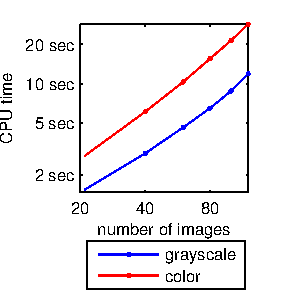
\includegraphics[width=5.5cm]{timing_studies_nimages}
%
\raisebox{5cm}{\textsf{B}}
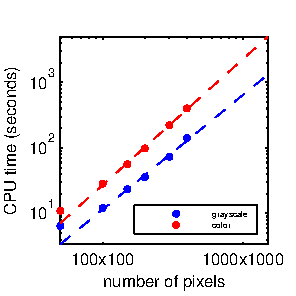
\includegraphics[width=5.5cm]{timing_studies_npixels}
%
\raisebox{5cm}{\textsf{C}}
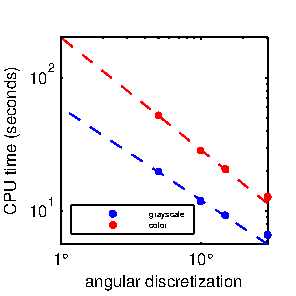
\includegraphics[width=5.5cm]{timing_studies_nrot}

\raisebox{1.75cm}{\textsf{D}}
{\renewcommand{\arraystretch}{1.5}
{ \textsf{ \small 
\begin{tabular}{ | p{2cm} | c | c | c | c | c | c | }
\hline
Data Set & 
Data Type & 
\parbox[c]{2cm}{ \centering Number of Channels} & 
\parbox[c]{2cm}{ \centering \vspace{.5\baselineskip} Number of Images \vspace{.5\baselineskip}} & 
\parbox[c]{2cm}{ \centering Number of Pixels} & 
\parbox[c]{2cm}{ \centering Angular Discretization} & 
\parbox[c]{2cm}{ \centering CPU time}  \\
\hline
{\em Drosophila} live~imaging & 2D & 1 & 40 & 100 $\times$ 100 & 10$^\circ$ & 3.2~sec \\ 
Zebrafish & 2D & 1 & 120 & 100 $\times$ 100 & 10$^\circ$ & 13~sec\\ 
{\em Drosophila} fixed images & 2D & 3 & 120 & 100 $\times$ 100 & 10$^\circ$ & 29~sec  \\ 
Wing disc & 3D & 3 & 46 & 100 $\times$ 100 $\times$ 21 & 10$^\circ$ & 12~sec  \\
 \hline
\end{tabular}}}}
\caption{Computational requirements for the presented methodology. (A) CPU time as a function of the number of images in the data set (for $100 \times 100$ pixel images, and $10^\circ$ angular discretization). Empirically, the CPU time is $\sim \mathcal{O}(n^{1.33})$ in number of images. (B) CPU time as a function of the number of pixels in the images (for $120$ images, and $10^\circ$ angular discretization). Empirically, the CPU time is $\sim \mathcal{O}(n^{1.83})$ in number of pixels. (C) CPU time as a function of the number of rotations (for $120$ images of $100 \times 100$ pixels). Empirically, the CPU time is $\sim \mathcal{O}(n^{-0.77})$ in the angular discretization. (D) The algorithm settings and computational requirements for the data sets analyzed. All times are reported for an Intel Core i7 2.93 GHz processor.}
\label{fig:cpu_time}
\end{figure*}

Manually ordering the images is nontrivial for researchers who are unfamiliar with the relevant developmental progression, and can be tedious and time-consuming for those who are.
%
In contrast, our method requires relatively little computational time.
%
The computational costs for our methodology are outlined in \fig~\ref{fig:cpu_time}.
%
The computational time is a function of the number of images in the data set, the number of pixels in each point, and the angular resolution to compute the pairwise rotations (see \SI). 
%
Furthermore, the computation of the pairwise rotational alignments, which accounts for the majority of the computational time, is trivially parallelizable for larger data sets.
%
Becasuse the computational cost increases with the image resolution, we chose to subsample all of our data sets to $100 \times 100$ pixels.
%
This resolution allowed us to rapidly analyze our data sets while still capturing all of the relevant developmental features.
%
However, as can be seen from the computational costs in \fig~\ref{fig:cpu_time}, it is feasible to use our algorithms to analyze higher-resolution images.

The requisite user intervention and parameter tuning required for our method is relatively minimal.
%
As a first step, images must be preprocessed so that the Euclidean distance between the pixels is informative.
%
Our software provides several preprocessing options (such as blurring, rescaling, and mean-centering), as well as some guidance for what options to select depending on the system of interest. 
%
Two algorithmic parameters, the angular discretization to compute the pairwise alignments and the diffusion maps kernel scale which determines which data points are ``close'' (see ~\fig~\ref{fig:schematics}A and \SI), must also be defined; we also provide some guidance on selecting these parameters.
%
We found that the results are robust to both of these parameters.
%
Overall, the tasks of image preprocessing and parameter selection are relatively simple compared to manual registration and ordering of images, and so this methodology is promising for much larger imaging data sets which are impractical to evaluate manually. 




\section*{Discussion}

Already at this point, the rate of collection of imaging data has surpassed the rate of manual image analysis.
%
This necessitates the development of automated methodologies to organize such large data sets. 
%
To the best of our knowledge, algorithmic approaches to these two tasks have been explored largely independently of each other. 
%
Temporal ordering of large-scale data which did not require registration was done in the context of molecular profiling studies, in which data are vectors describing the expression levels of different mRNA \citep{anavy2014blind, trapnell2014dynamics, gupta2008extracting}.
%
At the same time, temporal ordering of imaging data sets was done with a significant amount of human supervision and using registered images as a starting point \citep{yuan2014automated, surkova2008characterization}.  
%
%The task of image registration has been widely studied \citep{zitova2003image}, for applications such as face recognition \citep{rowley1998rotation}, medical image registration \citep{hajnal2010medical}, and texture classification \citep{greenspan1994rotation}.
%
In contrast to most of the existing registration approaches which rely on the knowledge of appropriate landmarks in the images \citep{ian1998statistical} (such as the eyes in face recognition applications \citep{zhao2003face}), algorithms based on angular synchronization can register images even in the absence of such information, making them relevant for a wide variety of applications. 
%
We have applied our methodology to several different proprotypical data sets in developmental biology; because our methodology only relies on computing distances between images,, we are confident it may be readily extended to many other data sets. 

We acknowledge that our methods, though general, do have some limitations. 
%
The first is that we require enough amount of data to sufficiently sample the developmental trajectory.
%
Therefore, for very small and/or very noisy data sets, our algorithms may fail. 
%
Second, the relevant developmental patterns and structures need to be large compared to the noise and the image resolution. 
%
In all of our examples, the relevant features, such as expression patterns and morphological structures, all span several pixels and are large compared to both the instrument noise and embryo-to-embryo variability. 
%
This means that the Euclidean distance is a good measure of similarity between images.
%
Our algorithms will fail for other imaging data sets which contain very fine scale structures,  as small perturbations in these fine-scale structures will result in large changes in the Euclidean distances. 
%
In such cases, one requires a more sophisticated distance metric, such as the Earth Mover's Distance \citep{...}, or image description, such as scattering transform coefficients \citep{...}, which are insensitive to such perturbations. 
%
Furthermore, as we have acknowledged, our methods as implemented cannot register full three-dimensional data with respect to rotations due to computational limitations. 
%
However, the algorithms presented here could be used for three-dimensional given an alternative method for computing pairwise alignments more efficiently (such as using image features or landmarks).

Unlike traditional statistical methods, our algorithms do not provide confidence intervals on predicted orderings, but could in principle be extracted from bootstrapping \citep{efron1979bootstrap}.
%
Furthermore, although our methods provide a temporal ordering for images, the provide no real-time information, neither do they provide a direction for the proposed ordering.
%
Determining which ``end'' of the trajectory is early and which is late is a post-processing task which requires {\em a priori} knowledge of the developmental dynamics. 
%
Furthermore, real-time information can only be extracted from either {\em a priori} knowledge of the rates of relevant developmental processes, or by making some assumption about the temporal sampling of the data set (e.g., the data set uniformly samples some given time window). 

Angular synchronization and vector diffusion maps have been used to reconstruct molecular shapes from cryo-electron microscopy images \citep{singer2012vector, zhao2014rotationally, singer2011viewing}.
%
Because of high levels of instrument noise in these data, thousands of images were needed for successful shape reconstruction. 
%
Based on the presented results, we expect that much smaller data sets may be sufficient for successful reconstruction of developmental trajectories from snapshots of fixed embryos.
%
In general, the size of the data set required for accurate registration and ordering is a function of the instrument noise, interembryo variability, and the complexity of the developmental dynamics.
%

Vector diffusion maps allow us to automatically register images, an essential task for many applications.
%
Simultaneously, the algorithm provides us with parameters to describe each image.
%
In the examples presented here, we have focused on ordering the images in time using the first vector diffusion maps coordinate.
%
In general, we can recover several parameters which concisely and comprehensively describe data set.
%
This parameterization can then be used for typical data analysis tasks, such as outlier detection and model fitting.
%
Data which comes from several different genetic backgrounds can be clustered according to their spatial expression patterns, and clustering can also be used to separate images into different developmental stages. 
%
Furthermore, images taken from different viewing directions can be analyzed, as the vector diffusion maps parameterization will organize the images according to the viewing angle.
%
Another direction for future work is related to the joint analysis of data sets provided by different imaging approaches, such as merging live imaging data of tissue morphogenesis with snapshots of cell signaling and gene expression from fixed embryos \citep{krzic2012multiview, ichikawa2014live, rubel2010coupling}.  
%
Given the rapidly increasing volumes of imaging data from studies of multiple developmental systems, we expect that dimensionality reduction approaches discussed in this work will be increasingly useful for biologists and motivate future applications and algorithmic advances. 
  

%% == end of paper:

%% Optional Materials and Methods Section
%% The Materials and Methods section header will be added automatically.

%% Enter any subheads and the Materials and Methods text below.


\section*{Materials and Methods}

\subsection*{{\em Drosophila} Experiments}
%
Oregon-R was used as wild type {\em Drosophila} strains. 
%
Embryos were collected and fixed at 22$^\circ$C. 
%
Monoclonal rabbit anti-dpERK (1:100, Cell signaling) and rat anti-Twist (1:500, a gift from Eric Wieschaus) were used to stain proteins of interest. 
%
DAPI (1:10,000, Vector Laboratories) was used to visualize nuclei, and Alexa Fluors (1:500, Invitrogen) were used as secondary antibodies. 
%
Histone-RFP strain was used to obtain time-lapse movie of gastrulating embryos at 22$^\circ$C. 
%
Embryos were loaded to the microfluidic device with PBST to keep them oxidized. 

\subsection*{{\em Drosophila} Microscopy}
%
Nikon A1-RS scanning confocal microscope, and the Nikon 60x Plan-Apo oil objective was used to image embryos. 
%
Embryos were collected, stained, and imaged together under the same microscope setting. 
%
End-on imaging was performed by using the microfluidics device described previously \citep{chung2010microfluidic}.
%
Images were collected at the focal plane $\sim$90~$\mathrm{\mu m}$ from the posterior pole of an embryo (see \fig~\ref{fig:DV_view}).  

\subsection*{Image preprocessing}

Images were subsampled, normalized, blurred, and centered prior to diffusion maps analysis to remove any variations due to the epxperimental and imaging framework. 
%
Details about the preprocessing operations applied to each imging data set are given in \SI. 


\subsection*{Software}
%
All algorithms and analysis were implemented in MATLAB\textsuperscript{\textregistered} (R2013b, The MathWorks, Natick, Massachusetts).
%
Code is available at \texttt{genomics.princeton.edu/stas/publications.html} under ``Codes and Data''. 

%\end{materials}



\subsubsection*{Acknowledgements}

The authors thank Fisun Hamaratoglu and Markus Affolter for providing the wing disc data. 
%
The authors thank Angela DePace, Granton Jindal, Adam Finkelstein,  Thomas Funkhouser, and John Storey for helpful discussions. 


\subsubsection*{Author contributions}
Scientific approaches were developed by C.J.D, B.L., H.L., A.S., S.Y.S, and I.G.K.
%
Experiments were performed by B.L.
%
Data analysis was performed by C.J.D. and B.L.
%
The manuscript was prepared and edited by C.J.D, B.L., H.L., A.S., S.Y.S, and I.G.K.

\subsubsection*{Funding}
C.J.D. was supported by the Department of Energy Computational Science Graduate Fellowship (CSGF), grant number DE-FG02-97ER25308, and the National Science Foundation Graduate Research Fellowship, Grant No. DGE 1148900.
%
B.L. and S.Y.S. were supported by the National Institutes of Health Grant R01GM086537. 
%
H.L. was supported by the National Science Foundation Grant Emerging Frontiers in Research and Innovation (EFRI) 1136913.
%
A.S. was supported by the Air Force Office of Scientific Research Grant
FA9550-12-1-0317.
%
I.G.K. was supported by the National Science Foundation (CS\&E program).


\bibliographystyle{development}
\bibliography{references}


\end{document}





